\documentclass{article}
\usepackage[dblblindworkshop,final]{neurips_2026}
\workshoptitle{AI for Science: Verification in the Age of AI Scientists}
\usepackage[utf8]{inputenc}
\usepackage[T1]{fontenc}
\usepackage{amsmath,amssymb,booktabs,microtype,graphicx,url,hyperref}
\usepackage{xcolor}
\usepackage{float}
% Original figure paths from the long-form LaTeX project.
\graphicspath{{figures/}}
% Canonical title: match the accepted OpenReview workshop submission exactly.
\title{Verifying When Black-Hole Hair Can Be Learned:\\Physical Identifiability, Generalization, and Observable Complementarity}
\author{Ariadna Uxue Palomino Ylla\\Nagoya University, Nagoya, Japan\\\texttt{ariadnaepy@gmail.com}}
\hypersetup{pdftitle={Verifying When Black-Hole Hair Can Be Learned: Physical Identifiability, Generalization, and Observable Complementarity},pdfauthor={Ariadna Uxue Palomino Ylla}}
\newcommand{\wq}{w_q}
\newcommand{\smin}{\sigma_{\min}}
\begin{document}
\maketitle
\begin{abstract}
Accurate parameter recovery from simulated observables need not imply identifiable physics or reliable extrapolation. We test these distinctions in a two-parameter Kiselev black hole benchmark with an exact null control: at $k=0$, the geometry is independent of $w_q$. Our verification combines local observable-Jacobian analysis, physical-system holdouts, conformal-coverage audits, and higher-resolution evaluation of frozen estimators. Adding photon geometry to leading-eikonal ringdown increases the median pointwise weakest-direction singular value by $4.54\times$ under the predefined feature normalization (paired finite-grid bootstrap 95\% interval $[4.28,4.94]$); redshift provides a separate complementary channel. Grouped identifiable-$w_q$ normalized mean absolute error (NMAE) improves from $0.3093$ for ringdown alone to approximately $0.087$ with photon geometry. A restricted observation-facing test removes latent photon-orbit descriptors: adding redshift to only $\Omega$ and $\lambda$ reduces grouped $w_q$ NMAE from $0.3886$ to $0.0985$. A non-learned nearest-model inverse supports complementarity. The targeted 321-phase forward audit meets its prespecified convergence criteria, yet tree-estimator prediction tails remain sensitive and an MLP exhibits severe directional extrapolation failures. The outcome is a controlled verification case study, not detector-level inference.
\end{abstract}
\section{Introduction}
Scientific inverse models can appear successful for the wrong reasons: training and test data may share physical information, observables may not distinguish the target parameters, or converged numerical inputs may still produce unstable predictions. These failure modes call for separate tests rather than a single accuracy score \citep{cranmer2020,ovadia2019}. Black hole spectroscopy makes the issue concrete: a predicted parameter is scientifically meaningful only if the chosen spacetime observables actually respond to it independently \citep{dreyer2004,cardoso2009}.

Here ``hair'' denotes the two Kiselev deformation parameters $(k,w_q)$ used in the benchmark, not an established violation of a black hole no-hair theorem. We use this controlled spacetime \citep{kiselev2003} because it supplies a ground-truth non-identifiable boundary. At $k=0$, all values of $w_q$ describe the same Schwarzschild metric. This lets us check whether a physical diagnostic correctly reports missing information, independently of any fitted estimator. Beyond that boundary, photon geometry and redshift improve the weakest parameter-response direction relative to leading-eikonal ringdown. Crucially, we also test whether this gain survives after removing latent photon-orbit quantities from the inverse inputs, keeping only leading-eikonal $\Omega$ and $\lambda$ plus selected redshift or sky summaries. Their impact on learned recovery must nevertheless be tested under physical holdouts and numerical refinement.


\section{Physical benchmark and verification protocol}
In geometrized units $M=1$, the Kiselev metric is
\begin{equation}
 ds^2=-f(r)dt^2+f(r)^{-1}dr^2+r^2d\Omega^2,\qquad f(r)=1-\frac{2}{r}-\frac{k}{r^{1+3\wq}}.
\end{equation}
Two feature comparisons are kept distinct throughout: the \emph{full theoretical-feature benchmark} includes latent orbit descriptors, whereas the \emph{restricted observation-facing test} deliberately removes them. The accepted $11\times11$ grid contains 121 systems with $k\in[0,0.0025]$ and $w_q\in[-0.7125,-0.45]$. Ringdown features are four leading-eikonal scalars derived from the unstable circular null orbit \citep{cardoso2009,konoplya2017}. In this approximation, $\Omega$ is the orbital frequency of a photon on that unstable circular orbit and $\lambda$ measures how rapidly a small displacement from it grows; the other two ringdown inputs describe the underlying orbit geometry. For the physical shooting observables, a timelike emitter with $r_p=8M$ and $r_a=12M$ is evolved over coordinate azimuth $\phi\in[\pi,3\pi]$; direct three-dimensional null rays are shot to a static observer at $(0,0,-80M)$. Phase-resolved impact parameter, signed sky coordinates, redshift, and timing are compressed into fixed per-system features. Failed phases are not filled or interpolated. The primary Jacobian archive uses 81 phases; a matched 161-phase archive is used in the extended inverse comparisons and convergence checks, and 321 phases are evaluated only for a prespecified 35-system stress set.

For an observable vector $\mathbf O(\theta)$, $\theta=(k,w_q)$, we analyze the scaled Jacobian
\begin{equation}
 J_{ij}=\frac{\Delta\theta_j}{s_i}\frac{\partial O_i}{\partial\theta_j},\quad \Delta k=0.0025,\quad \Delta w_q=0.2625,
\end{equation}
where $s_i$ is the nominal grid's q95--q05 feature range. Its minimum singular value $\smin$ measures the weakest local parameter direction; $\kappa(J)=\sigma_{\max}/\smin$ measures anisotropy. These magnitudes are normalization-dependent. At $k=0$, $\partial_{w_q}f=0$ exactly, hence the $w_q$ column vanishes and $\smin=0$. Full rank at finite $k$ need not imply recovery at finite precision \citep{raue2009,villaverde2016}.

All learning uses one feature record per physical system, not a separate training example for each phase. Five seeds define random interpolation, two blocked $3\times3$ group layouts, and four directional edge holdouts. Training, calibration, and test records are disjoint; physical-equivalence overlap among the nominal $k=0$ records is audited separately in Appendix~\ref{app:coverage}. Preprocessing is fitted on training data only; conformal residual quantiles are fitted on the disjoint calibration subset. The 11 nominal $k=0$ rows share a physical equivalence class: they contribute to $k$ scoring but not ordinary $w_q$ error. An additional collapsed-class sensitivity analysis checks this design. Models are histogram gradient boosting (HGB), random forest (RF), and target-scaled multilayer perceptron (MLP); their role is to expose distinct estimator failures, not to introduce a new architecture \citep{breiman2001,pedregosa2011}. NMAE divides MAE by the full physical parameter span.

\section{Identifiability and observable complementarity}
We first report the \emph{full theoretical-feature benchmark}, whose four ringdown scalars include latent photon-orbit descriptors. Table~\ref{tab:complementarity} and Fig.~\ref{fig:complementarity} describe this benchmark; the restricted experiment is reported separately in Sec.~\ref{sec:restricted}. The decisive physical distinction is between a large observable response and independent parameter-response directions. Across 110 finite-$k$ systems, augmenting ringdown with photon geometry raises the median of pointwise $\smin$ ratios by $4.54\times$ and improves the median pointwise conditioning ratio by $2.28\times$. Redshift also improves these quantities ($3.29\times$ and $2.27\times$). The Jacobian improvement is not simply an effect of a particular learned architecture.

\begin{table}[H]
\caption{\textbf{Full theoretical-feature benchmark}, including latent ringdown descriptors. Jacobian medians use the nominal 81-phase archive; inverse NMAE uses the matched 161-phase comparison. These results are distinct from the restricted experiment in Table~\ref{tab:restricted}.}
\label{tab:complementarity}
\centering\small
\begin{tabular}{lrrrr}
\toprule
Feature set & median $\smin$ & median $\kappa$ & grouped NMAE & directional NMAE\\
\midrule
Ringdown & 0.2782 & 6.6112 & 0.3093 & 0.3011\\
Ringdown + redshift & 0.9459 & 3.6107 & 0.0991 & 0.1922\\
Ringdown + photon geometry & 1.2326 & 4.0731 & 0.0865 & 0.2048\\
\bottomrule
\end{tabular}
\end{table}

\begin{figure}[t]
\centering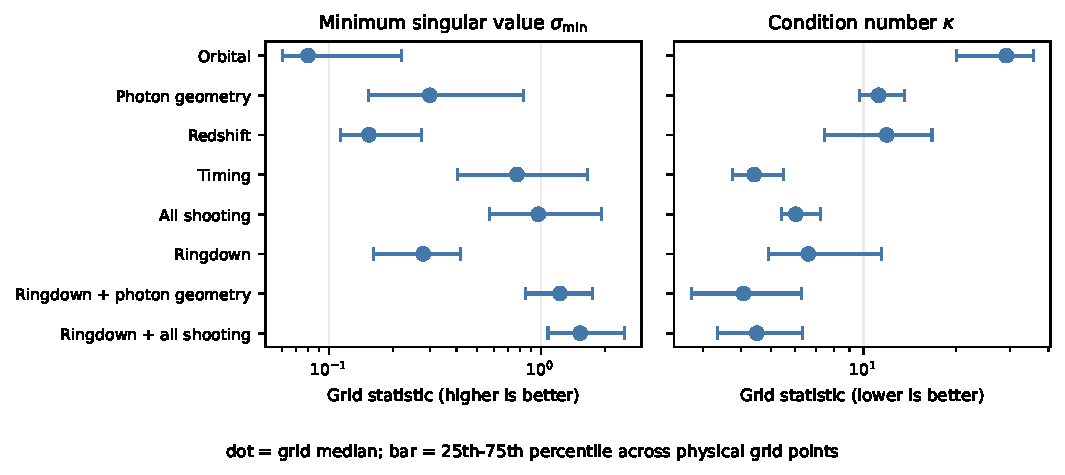
\includegraphics[width=.91\linewidth]{physical_observable_complementarity_landscape.pdf}
\caption{Finite-grid weakest-direction sensitivity and conditioning across observable families. Bars denote grid-point interquartile ranges, not observational uncertainties.}
\label{fig:complementarity}
\end{figure}

The bootstrap interval for the photon-geometry weakest-direction gain is $[4.28,4.94]$; for the conditioning improvement it is $[1.84,2.63]$, resampling the eligible finite-$k$ systems. Observable-scaling checks (IQR, standard-deviation, and family balancing) preserve the qualitative improvement but change the numerical factors. The observation-facing restriction below tests whether the main conclusion relies on latent geometric descriptors. The full scaling comparisons are in Appendix~\ref{app:extra}.


\subsection{Recovery without latent geometric inputs}\label{sec:restricted}
The original ringdown benchmark contains four scalars, including photon-orbit descriptors not independently measured in ringdown observations. We therefore remove $\Delta r$ and $r_{\mathrm{ph}}$ and retain only the leading-eikonal quantities $\{\Omega,\lambda\}$. We then add either the nine phase summaries of redshift $z$, or the 18 summaries of signed observer-sky coordinates $\{\alpha,\beta\}$; impact-parameter, orbital, and timing features are excluded. This tests whether a reduced set of physically motivated, potentially observation-linked summaries retains useful information \emph{within the simulated benchmark}; it does not establish that a detector could measure these summaries with the required precision.

\begin{table}[H]
\caption{\textbf{Restricted observation-facing benchmark (no latent photon-orbit inputs).} Finite-$k$ Jacobian medians use nominal 81-phase features; identifiable-$w_q$ NMAE uses the matched 161-phase inverse tests with the same predefined holdouts. These are simulated feature summaries, not detector measurements.}
\label{tab:restricted}
\centering\small
\begin{tabular}{lrrrr}
\toprule
Inverse inputs & median $\smin$ & median $\kappa$ & grouped NMAE & directional NMAE\\
\midrule
$\Omega,\lambda$ only & 0.0097 & 136.69 & 0.3886 & 0.4239\\
$+\,z$ summaries & 0.6215 & 4.47 & 0.0985 & \textbf{0.1750}\\
$+\,\alpha,\beta$ summaries & 0.6999 & 4.89 & 0.0904 & 0.2179\\
$+\,z,\alpha,\beta$ summaries & 0.7310 & 5.59 & \textbf{0.0807} & 0.1949\\
\bottomrule
\end{tabular}
\end{table}

With only $\Omega$ and $\lambda$, the weakest Jacobian direction is small and grouped recovery of $w_q$ is poor. Adding redshift alone reduces grouped NMAE from $0.3886$ to $0.0985$ and directional NMAE from $0.4239$ to $0.1750$; no $r_{\mathrm{ph}}$, impact parameter, or sky-coordinate input is required for this gain. Signed sky coordinates provide a separate improvement. Combining redshift and sky gives the best grouped aggregate ($0.0807$), but redshift alone yields the lowest directional error ($0.1750$). Thus additional feature families need not monotonically improve extrapolation. The corresponding non-learned nearest-model comparison also improves from $0.4238$ to $0.1417$ (grouped) after adding redshift, supporting information complementarity beyond the learned architectures. These are \emph{observation-facing} inputs: $\Omega,\lambda$ are leading-eikonal descriptors, and the redshift and sky features are generated from idealized trajectories without a measurement likelihood or detector noise.

\section{Inverse recovery and uncertainty under shift}
Random interpolation is easier than physical holdout. For the primary aggregate, ringdown random NMAE is $0.0361/0.1688$ for $k$/identifiable $w_q$, increasing to $0.0485/0.3093$ under grouped holdout. With photon geometry, grouped scores improve to $0.0457/0.0875$ in the primary aggregate. For identifiable $w_q$, the primary 81-phase aggregate gives $0.0875$; the matched 161-phase comparison in Table~\ref{tab:complementarity} gives $0.0865$. That matched comparison also shows that redshift improves the difficult $w_q$ direction. Directional extrapolation remains challenging even for augmented features.

\begin{figure}[t]
\centering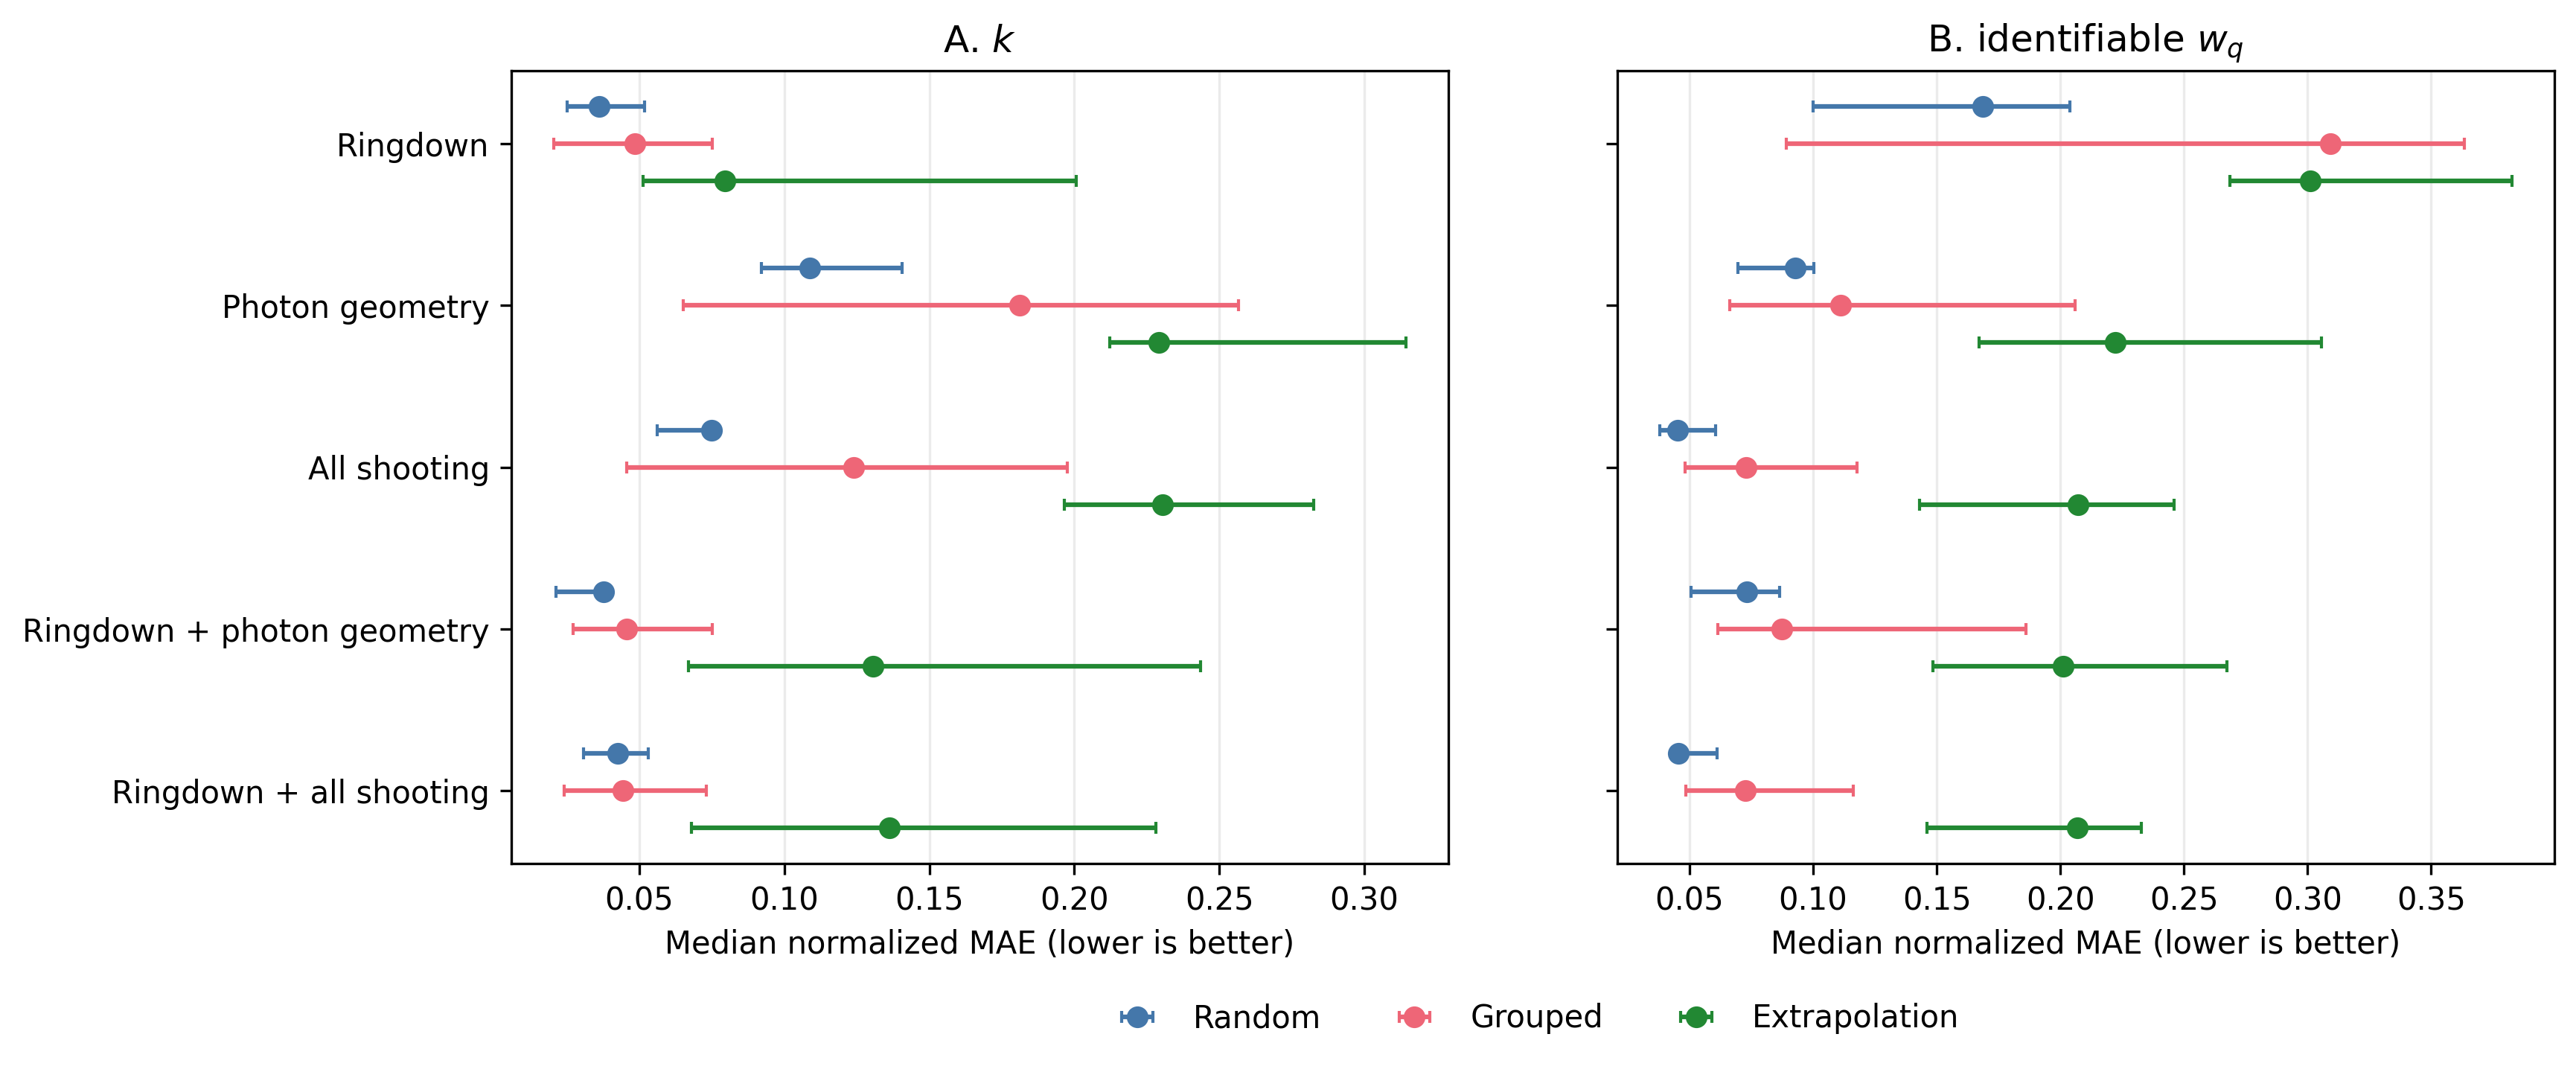
\includegraphics[width=.84\linewidth]{physical_ml_protocol_comparison.png}
\caption{Random, grouped, and directional inverse NMAE across primary feature families. Points are medians of stored summary-row medians; bars show 25th--75th percentiles of underlying records across applicable folds, seeds, models, and directions. The different aggregation levels are intentional, and directional results remain separately archived.}
\label{fig:protocols}
\end{figure}

A non-learned nearest-physical-model inverse provides a direct cross-check: grouped identifiable-$w_q$ NMAE falls from $0.2208$ for ringdown to $0.1481$ with photon geometry (and $0.1585$ with redshift). A local Jacobian inverse obtains favorable median errors but yields 1,315 out-of-domain predictions among 9,950, demonstrating that locally good inversion need not be globally safe. These baselines reinforce observable complementarity without asserting the superiority of any inverse method.

Empirical 90\% split-conformal coverage for $k$/identifiable $w_q$ declines from $0.892/0.965$ for random splits to $0.722/0.851$ for grouped holdout and $0.509/0.660$ for directional evaluation. These are medians across overlapping archived evaluation summaries, not independent Bernoulli trials. Selected dispersion summaries appear in Appendix~\ref{app:coverage}; unit-level Wilson intervals are provided in the archived evaluation tables. Coverage under directional shift is descriptive, as standard exchangeability conditions do not persist \citep{angelopoulos2021,tibshirani2019}.

\section{Forward convergence versus frozen-estimator robustness}
We ask two separate questions: do finer simulations change the input features appreciably, and do those changes destabilize an already-trained inverse model? We quantify the first question by comparing phase resolutions with
\begin{equation}
 \delta_i=\frac{|F_i^{(N_2)}-F_i^{(N_1)}|}{\max(s_i,10^{-12})}.
\end{equation}
A feature--point change is classified as converged for $\delta_i\leq0.01$, marginal for $0.01<\delta_i\leq0.05$, and unresolved above $0.05$ (also for missing/non-finite values). The uniform 81-to-161 comparison leaves 240 of 9,317 comparisons above $0.05$. The targeted 35-point 161-to-321 audit, chosen before seeing 321-phase outcomes, meets its prespecified forward criteria: median change $1.963\times10^{-4}<0.001$, p95 $7.234\times10^{-3}<0.01$, no unresolved comparison, unchanged ringdown, no systematic feature-family trend, and preserved Jacobian rank. Its within-selected-set resolution-shift rankings have Spearman correlations 1.000 (maxima) and 0.997 (p95), but this is not a full-grid 321-phase convergence claim.

\begin{figure}[t]
\centering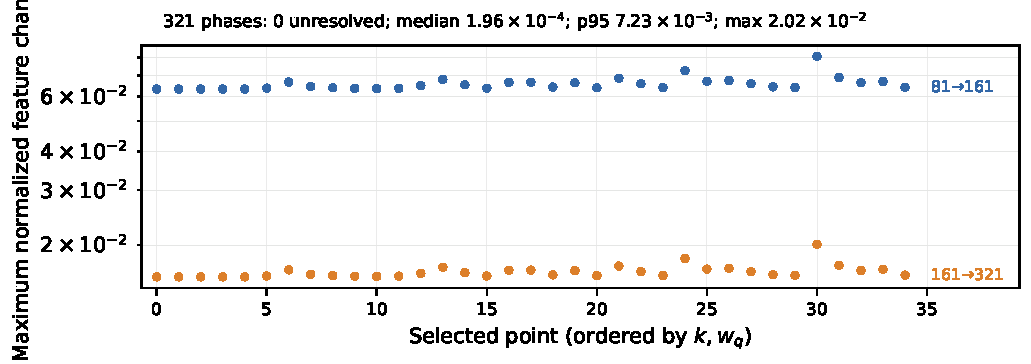
\includegraphics[width=.86\linewidth]{resolution_robustness_compact.pdf}
\caption{Resolution changes for the 35 selected systems. Each plotted point is the \emph{maximum across features at one system} (blue: 81--161 phases; orange: 161--321). The annotation gives \emph{pooled feature--point} median, p95, and maximum for 161--321, which are different statistics. Selection and convergence claims apply only to these 35 systems at 321 phases.}
\label{fig:resolution}
\end{figure}

Passing the forward test does not certify frozen estimators. HGB and RF median shifts are zero but their p95 prediction shifts are $0.08122$ and $0.08509$, exceeding the prespecified tree tolerance of $0.03$. Maximum identifiable-$w_q$ shifts reach $0.30593$ and $0.27053$. The MLP is smoother under local phase substitution (p95 shift $0.008223$), yet 409 of its 410 catastrophic directional records already occur at 161 phases. This separates tree split-crossing sensitivity from MLP extrapolation instability. Thus the prespecified decision remains \emph{forward acceptance, inverse-estimator robustness failure}.

\begin{figure}[t]
\centering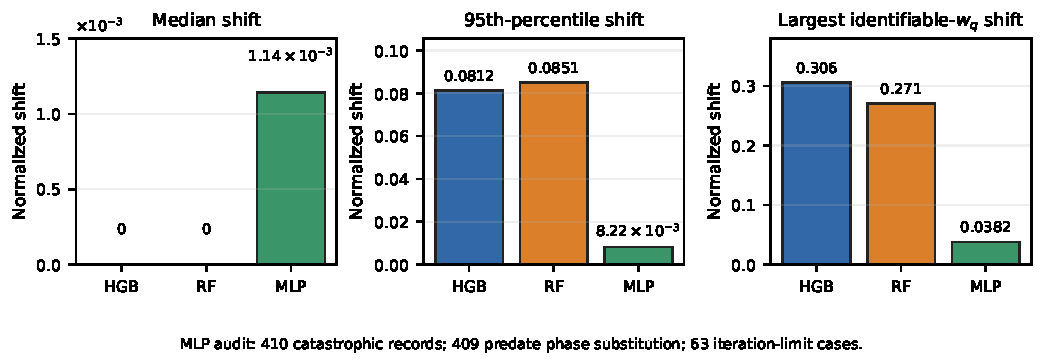
\includegraphics[width=.85\linewidth]{targeted_estimator_robustness_compact.pdf}
\caption{Frozen estimator changes after matched 321-phase substitution: negligible median tree shifts can coexist with consequential prediction tails.}
\label{fig:estimator}
\end{figure}

\section{Discussion and verification guidance}
The experiment supports a simple order of operations. Full theoretical features and restricted observation-facing summaries are separate experiments; the latter establish useful recovery with fewer latent inputs, not constraints from actual observations. First, test analytic invariances and parameter rank: a claim of $w_q$ information at $k=0$ must fail. Next, evaluate whether another observable family supplies a distinct response direction, under an explicit normalization. Then test recovery with physical systems withheld and with directional shifts, reporting uncertainty empirically where exchangeability is absent. Finally, test independently converged features on \emph{frozen} fitted estimators and report tails, not only medians. A failed layer calls for a different remedy: new observables for weak physical identifiability, wider training support for distribution shift, and more stable inverse estimators for numerical perturbation sensitivity.

This is a proof-of-concept on one static spherical spacetime, one direct photon branch, finite grid coverage, leading-eikonal ringdown and idealized geometric observables. We make no observational strain or imaging likelihood claim, no proof of continuous global injectivity, and no universal threshold for a ``good'' singular value. Exact verification controls may be harder to identify in other problems; where unavailable, independent physical limits and non-learned inverse checks provide partial alternatives. The research release is \url{https://doi.org/10.5281/zenodo.23191840}; all original fitted-estimator files have been recovered and their replay validated locally, but their separate public archive is still pending (Appendix~\ref{app:extra}). Future investigations should test finite-multipole signals and observation-level uncertainties rather than infer detector constraints from this benchmark.

\section{Conclusion}
Identifiability, train--test support, uncertainty coverage, forward convergence, and inverse stability are distinct scientific obligations. Photon geometry and redshift improve distinguishability and grouped inverse recovery in this Kiselev benchmark, with non-learned checks supporting the direction of the effect. The effect persists when latent photon-orbit descriptors are excluded: even $\{\Omega,\lambda\}$ plus redshift summaries substantially outperforms the restricted ringdown-only baseline. The targeted forward calculation converges under its declared criteria, while archived inverse estimators retain significant failures. A trustworthy verification report must state both outcomes.

\section*{Data and code availability}
Derived data, code, split assignments, and numerical checks are described in the archived research release \url{https://doi.org/10.5281/zenodo.23191840}. The versioned configurations and prediction tables permit independent recalculation of reported aggregates. All 5,520 original serialized fitted estimators have now been located and replay-validated to a declared numerical tolerance; they are not yet in a public permanent archive. See Appendix~\ref{app:extra} for scope and availability.

\begin{thebibliography}{20}\setlength{\itemsep}{0pt}
\bibitem[Angelopoulos and Bates(2021)]{angelopoulos2021} A.~N. Angelopoulos and S.~Bates. A gentle introduction to conformal prediction and distribution-free uncertainty quantification. 2021.
\bibitem[Breiman(2001)]{breiman2001} L. Breiman. Random forests. \emph{Machine Learning}, 45:5--32, 2001.
\bibitem[Cardoso et~al.(2009)]{cardoso2009} V. Cardoso, A.~S. Miranda, E. Berti, H. Witek, and V.~T. Zanchin. Geodesic stability, Lyapunov exponents and quasinormal modes. \emph{Phys. Rev. D}, 79:064016, 2009.
\bibitem[Cranmer et~al.(2020)]{cranmer2020} K. Cranmer, J. Brehmer, and G. Louppe. The frontier of simulation-based inference. \emph{PNAS}, 117:30055--30062, 2020.
\bibitem[Dreyer et~al.(2004)]{dreyer2004} O. Dreyer et~al. Black-hole spectroscopy: testing general relativity through gravitational-wave observations. \emph{Class. Quantum Grav.}, 21:787--804, 2004.
\bibitem[Kiselev(2003)]{kiselev2003} V.~V. Kiselev. Quintessence and black holes. \emph{Class. Quantum Grav.}, 20:1187--1198, 2003.
\bibitem[Konoplya and Stuchl\'{\i}k(2017)]{konoplya2017} R.~A. Konoplya and Z. Stuchl\'{\i}k. Are eikonal quasinormal modes linked to the unstable circular null geodesics? \emph{Phys. Lett. B}, 771:597--602, 2017.
\bibitem[Ovadia et~al.(2019)]{ovadia2019} Y. Ovadia et~al. Can you trust your model's uncertainty? Evaluating predictive uncertainty under dataset shift. \emph{NeurIPS}, 32, 2019.
\bibitem[Pedregosa et~al.(2011)]{pedregosa2011} F. Pedregosa et~al. Scikit-learn: Machine learning in Python. \emph{JMLR}, 12:2825--2830, 2011.
\bibitem[Raue et~al.(2009)]{raue2009} A. Raue et~al. Structural and practical identifiability analysis of partially observed dynamical models by exploiting the profile likelihood. \emph{Bioinformatics}, 25:1923--1929, 2009.
\bibitem[Tibshirani et~al.(2019)]{tibshirani2019} R.~J. Tibshirani et~al. Conformal prediction under covariate shift. \emph{NeurIPS}, 32, 2019.
\bibitem[Villaverde et~al.(2016)]{villaverde2016} A.~F. Villaverde, A. Barreiro, and A. Papachristodoulou. Structural identifiability of dynamic systems biology models. \emph{PLOS Computational Biology}, 12:e1005153, 2016.
\end{thebibliography}
\appendix
\section{Audit definitions and sensitivity results}\label{app:extra}
\paragraph{Feature specification.} Four ringdown scalars are augmented by 27 photon-geometry summaries, nine redshift summaries, 20 orbital quantities, and 17 timing quantities. Each phase series is summarized by fixed means, amplitudes, reference values where defined, and low-harmonic sine/cosine coefficients. The primary Jacobian uses q95--q05 feature scales and full parameter spans. The finite-$k$ pointwise median photon-geometry gains under IQR, population-standard-deviation, and feature-family-balanced scaling are $5.88$, $3.76$, and $2.95$ for $\smin$ (versus $4.54$ nominal). They are scale-dependent, while the direction of the gain remains consistent.
\paragraph{Observation-facing restriction.} Table~\ref{tab:restricted} reports the restricted recovery and finite-$k$ Jacobian results. Redshift and signed sky coordinates are tested as separate phase-summary families, not as raw individual measurements. This restriction excludes latent photon-sphere and impact-parameter inputs, but neither a detector response nor an observational noise model is included.
\paragraph{Traditional inverse baselines.} For ringdown plus photon geometry, nearest-model grouped identifiable-$w_q$ NMAE is $0.1481$ and local Jacobian grouped NMAE is $0.0454$. The latter is a median-only summary: 1,315 of 9,950 local-Jacobian predictions leave the studied physical domain without clipping.
\paragraph{Estimator configurations and split protocol.}
The physical-shooting validation uses five fixed seeds (2026--2030), a 20\% random test fraction, a 20\% calibration fraction of the remaining systems, two shifted $3\times3$ block layouts, and four directional tests withholding three levels of $k$ or $w_q$. Histogram gradient boosting (HGB) uses \texttt{max\_iter=180}, \texttt{learning\_rate=0.06}, \texttt{max\_leaf\_nodes=15}, and \texttt{l2\_regularization=0.1}. Random forest uses 120 trees, maximum depth 8, and minimum leaf size 2. The MLP uses two hidden layers of widths $(32,16)$, \texttt{alpha=0.01}, at most 600 iterations, early stopping, and \texttt{n\_iter\_no\_change=30}. Its inputs and targets are standardized from training data only. The restricted observation-facing comparison reuses the registered split assignments and models and sorts physical-system identifiers before fitting to eliminate training-row-order ambiguity. See the versioned configuration \url{https://github.com/Uxuee/black-hole-hair-ml/blob/main/configs/physical_shooting_ml_validation.yaml} and experiment script \url{https://github.com/Uxuee/black-hole-hair-ml/blob/main/scripts/observation_facing_sensitivity.py}.
\paragraph{Reproducibility boundary.}
Archived feature, split, prediction, and summary tables permit independent recalculation of the reported aggregates without recovering the fitted estimators. Re-evaluating the \emph{same frozen fitted models} on alternative phase-resolution features requires their serialized estimator objects, including fitted preprocessing. A subsequent local audit recovered all 5,520 original fitted estimators (809.3 MiB), including fitted preprocessing. Replay of 95,520 archived 161-phase predictions and 30,672 predictions at each of the targeted 161- and 321-phase resolutions showed no mismatches at tolerance $10^{-12}+10^{-12}|\hat y|$; no retraining was performed. The model release package has been validated but is not yet publicly deposited. Until publication, independently recalculating aggregate statistics from archived tables and independently replaying the original fitted models have different public availability levels. The provenance and known model-file limitation are disclosed at \url{https://github.com/Uxuee/black-hole-hair-ml/blob/main/reviewer/_revision_2026_10/step07_presentation/reproducibility_matrix.csv}.
\enlargethispage{8\baselineskip}
\section{Coverage and $k=0$ equivalence sensitivity}\label{app:coverage}
The reported 90\% conformal coverage is the median across stored model--feature summaries. The row-level IQR for directional $k$ coverage is $[0.311,0.689]$ and for directional identifiable-$w_q$ coverage $[0.585,0.844]$. Evaluation units share physical systems and do not support one pooled binomial confidence interval. Of 115 predefined splits, nominal $k=0$ records occur in both training and testing in 45, and in training and calibration in 96. Collapsing all 11 Schwarzschild records to one equivalent record changes grouped identifiable-$w_q$ NMAE from $0.0875$ to $0.0859$, while its conformal coverage changes from $0.851$ to $0.763$. This is a sensitivity analysis, not a replacement for the prespecified primary splits.
\section{Resolution-audit scope}
The 35 preselected systems combine earlier feature/estimator stress rankings, boundary and central grid systems, directional representatives, conditioning extremes, and grouped-block representatives. All 35 complete at 321 phases. The frozen tree thresholds are median shift $<0.005$, p95 $<0.03$, maximum identifiable-$w_q$ shift $<0.1$ (subject to the recorded unresolved-feature rule), and aggregate NMAE change $<0.02$. These are separate from forward tolerances. Selection based on 161-phase information and within-subset rank agreement do not certify the other 86 grid systems at 321 phases.
\end{document}
